%\subsection{FeSe diatomic molecule (NE-DMD)}
\subsection{FeSe diatomic molecule}
\label{subsection:fese}
Transition metal systems are an especially difficult case for most electronic structure methods, and therefore, are an 
important test case for DMD. 
Diffusion Monte Carlo (DMC) is particularly useful in transition-metal systems, where is has been shown to improve the description of energy gaps for the types of orbital excitations used to sample the Hilbert space~\cite{Foyevtsova2014, Wagner_Abbamonte, Zheng2015, Wagner2016}.
Given the expense of large DMC calculations, finding models consistent with DMC would be valuable for studying extended transition metal systems. 
Additionally, transition metal systems involve competing interactions that can give rise to novel phenomena. 
Utilizing matching pursuit and DMD to find minimal descriptions can offer a way to quantify the relative importance of different interactions.

As a test of DMD for transition metal systems, we consider an FeSe diatomic molecule with atomic separation 2.43 \AA~in the $z$-direction.
To our knowledge, this FeSe diatom does not exist in nature, but nevertheless serves as a simple illustration of a model for the interaction between a transition metal and a ligand. 
The bond distance is chosen to match the unconventional superconductor, FeSe~\cite{kumar_crystal_2010}, and therefore offer insight into a model description for that system in future calculations.

We consider a multiband Hubbard model including one iron $s$, five iron $d$ states, and three selenium $p$ states:
\begin{align}
  H 
  &=
  \epsilon_{xy} \sum_{\eta} (n^{d_{xy}}_{\eta}  + n^{d_{x^2-y^2}}_{\eta})
  +
  \epsilon_s \sum_{\eta} n^{s}_{\eta} 
  +
  \epsilon_{p_{z}} \sum_{i,\eta} n^{p_{z}}_{i,\eta} 
  \nonumber \\
  &+ 
  t_{\sigma,d} \sum_{\eta} \left( d_{z^2,\eta}^{\dagger} p_{z,\eta} + \text{h.c.} \right)
  +
  t_{\sigma,s} \sum_{\eta} \left(s_{\eta}^{\dagger}  p_{z,\eta} + \text{h.c.} \right)
  \nonumber \\
  &+
  U_d \sum_{i} n^{d}_{i,\uparrow} n^{d}_{i,\downarrow} 
  +
  J_d \sum_{i\ne j} S_i \cdot S_j
  +
  E_0. \label{eq:fesemodel}
\end{align}
Here, $\eta$ represents the spin index and $i$ represents orbital index.
The $\epsilon_i$ terms represent single-particle orbital energies, while the $U_d$ is an on-site interaction among the $d$ orbitals and the $J_d$ is a Hund's coupling among the $d$ orbitals.
$E_0$ is an overall energy shift compared to the \textit{ab initio} hamiltonian.
This set of parameters was chosen based on the matching pursuit method described in Sec.~\ref{sec:theory}.
We considered the set of 21 symmetry allowed $\epsilon$, $t$, $U$, and $J$ parameters. 
For this demonstration, we add parameters one at a time until the RMS error drops by less than 0.05 eV. 
With this criteria, the final RMS error is 0.61 eV, the final coefficient of determination ($R^2$) is 0.84, and the next parameter in the algorithm reduces the $R^2$ by less than 0.01.
For example, $U_p$, an on-site interaction for the Se $p$-electrons, does not correlate strongly enough with the residuals, and is not added included before the algorithm halts.
The states sampled consisted of singles and doubles excitations from PBE0 calculations with total spin 0, 2, and 4, which were then relaxed via a DMC projection.
243 states fit within an energy window of 8 eV from the ground state, and were selected as the low energy space.
Out of these states, 8 states because the sum of all occupation descriptors was more than 0.5 less than the number of electrons.
These states generally have a significant iron $p$ component relative to the ground state, and therefore were excluded, as they are not describable without several additional parameters describing the iron $p$ states.

\begin{figure*}
  \centering
  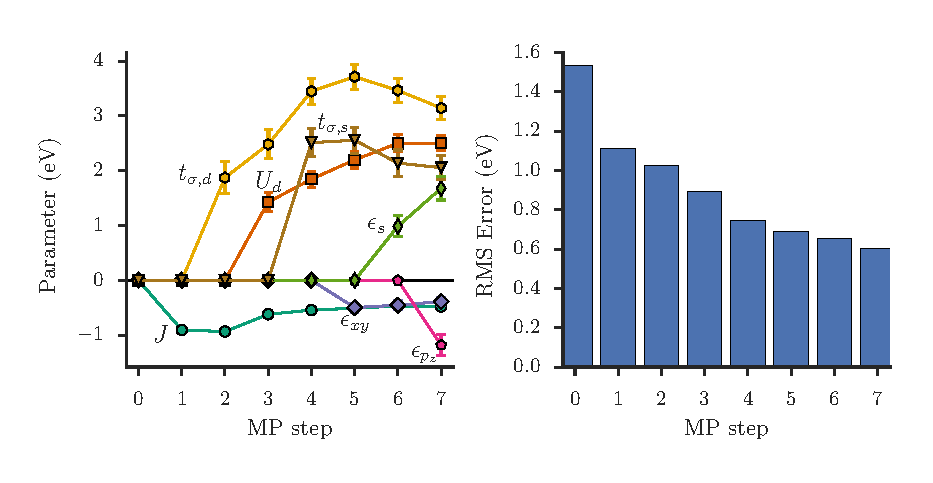
\includegraphics[width=0.8\textwidth]{./Figures/fese.eps}
  \caption{
    \label{fig:fese} 
    (A) Parameter values for each fit generated in the MP algorithm, labeled at the step where they are included in the model. 
    A zero value implies that parameter is not yet added to the model.
    The sign of $J$ is consistent with Hund's rules, and the signs of $t_{\sigma,d}$ and $t_{\sigma,s}$ are consistent with Se being located in positive $z$ with respect to Fe. 
    The $\epsilon_i$ states adjust the energies of the single particle orbitals relative to the energy of the other orbitals.
    (B) RMS error of each model generated by MP as the algorithm includes parameters. 
    MP tends to add parameters that reduce the error most significantly first. 
    $J$ correlates most with the error initially, is chosen first, and decreases error the most.
  }
\end{figure*}

Applying the MP approach to the system produced reasonable parameter estimates, and suggested the Hund's coupling to be an important component of this model.
Analysis of the MP results are shown in Fig.~\ref{fig:fese}. 
Fig.~\ref{fig:fese}(a) and (b) show the evolution of the parameters and RMS error of the fit as additional parameters are added.
All previous parameters may change at each step because the entire model is refitted with each iteration.
The parameters are smoothly varying with the inclusion of new parameters, and generally take reasonable values.
The matching pursuit algorithm would suggest that minimal models can be built by disregarding the descriptors added in later steps.
In this approach, $J$ is considered the most important parameter in the model, and an absolute minimal model for the system would be $H_\text{minimal} = E_0 + J_d \sum_i S_i \cdot S_j$. 
Such a model would have a RMS error 1.11 eV. 
According to matching pursuit the next most important interactions to include are (1) hopping between $d_{z^2}$ and $p_z$, (2) on-site $d$ Coulomb interactions, and (3) hopping between the $4s$ and the $p_z$, and so on. 
Including these degrees of freedom brings the RMS error to 0.75 eV.
In this way MP would suggest that the most important interactions in the system are Hund's coupling, hopping with Se, and on-site Coulomb repulsion, in that order.
This observation is consistent with the several studies in the literature, which find Hund's coupling in bulk FeSe to be an important part of its description~\cite{demedici_hunds_2011,de_medici_janus-faced_2011,georges_strong_2013,busemeyer_competing_2016}.
